\section{VPN on Windows}

Setting up a VPN on Windows is very easy once you have your account
details ready. Let's assume have your credentials from your VPN provider
for L2TP/IPSec connection ready. This information should contain the
following:

\begin{itemize}
\item
  Username, ex. \verb!bill2!
\item
  Password, ex. \verb!verysecretpassword!
\item
  VPN server, ex. \verb!tunnel.greenhost.nl!
\item
  A Pre-Shared-Key or Machine-certificate
\end{itemize}
\subsection{Setup}

\begin{enumerate}[1.]
\item
  Before getting started, please be sure you've read the paragraph
  ``testing before and after account set up'', this way you will be able
  to validate if your connection is actually working after set up.
\item
  We need to go to the ``Network and Sharing Center'' of Windows to
  create a new VPN connection. We can access this center easily by
  clicking on the network icon next to the systemclock en click on
  ``open Network and Sharing Center''
\end{enumerate}
\begin{figure}[htbp]
\centering
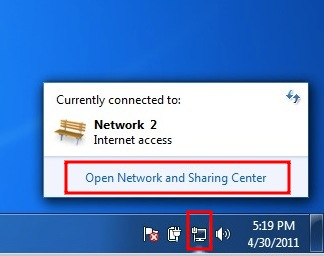
\includegraphics{vpn_windows_01.jpg}
\caption{VPN on Windows}
\end{figure}

\begin{enumerate}[1.]
\setcounter{enumi}{2}
\item
  The ``Network and Sharing Center'' will popup. You will see some
  information about your current network. Click on ``Connect to a
  network'' to add a VPN connection.
\end{enumerate}
\begin{figure}[htbp]
\centering
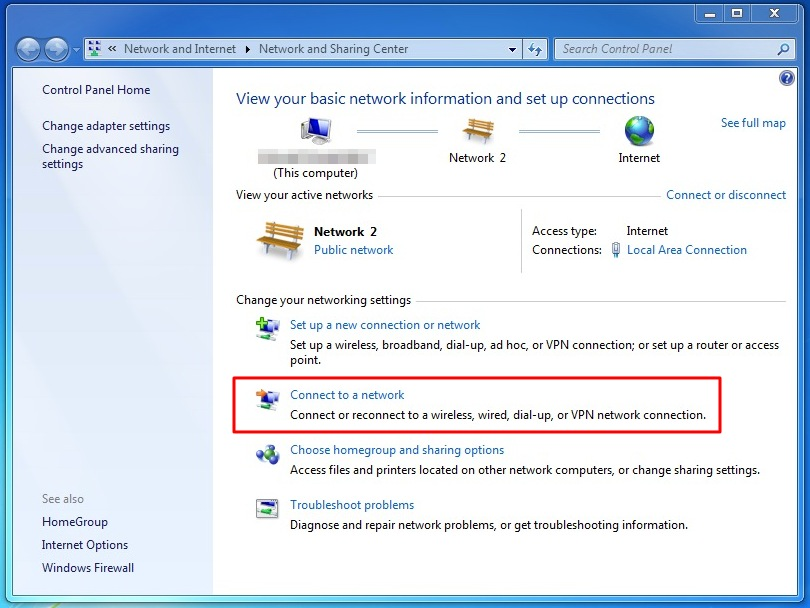
\includegraphics{vpn_windows_02.jpg}
\caption{VPN on Windows}
\end{figure}

\begin{enumerate}[1.]
\setcounter{enumi}{3}
\item
  The wizard to setup a connection will popup. Choose the option to
  ``connect to a workplace'', which is Microsoft's way of naming a VPN
  connection.
\end{enumerate}
\begin{figure}[htbp]
\centering
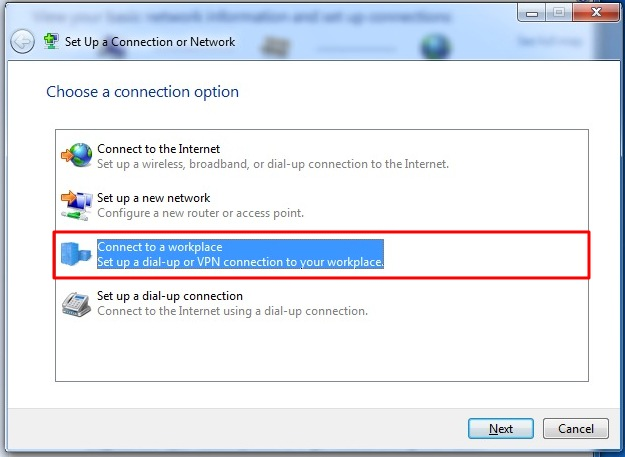
\includegraphics{vpn_windows_03.jpg}
\caption{VPN on Windows}
\end{figure}

\begin{enumerate}[1.]
\setcounter{enumi}{4}
\item
  The next screen asks us if we want to use our Internet connection or
  an old-skool phone line to connect to the VPN. Just choose the first
  option then.
\end{enumerate}
\begin{figure}[htbp]
\centering
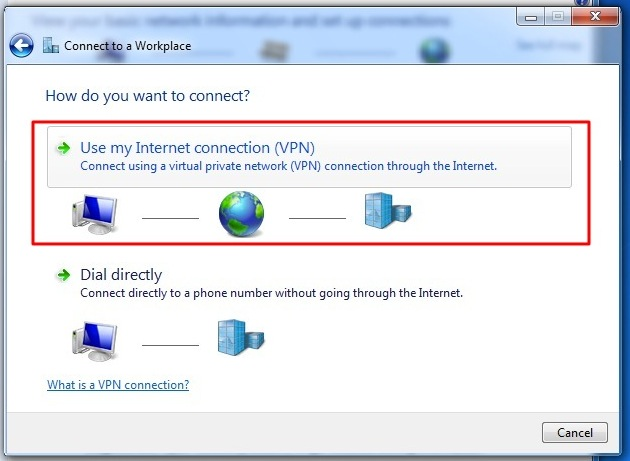
\includegraphics{vpn_windows_04.jpg}
\caption{VPN on Windows}
\end{figure}

\begin{enumerate}[1.]
\setcounter{enumi}{5}
\item
  The next screen asks for the connection details. Enter here the server
  of your VPN-provider (called ``Internet address'' in this dialog). On
  the bottom please check the box ``Don't connect now; just set it up''.
  Using this option the connection will be automatically saved and it's
  easier to control extra settings. If this is all done, hit the
  ``next'' button
\end{enumerate}
\begin{figure}[htbp]
\centering
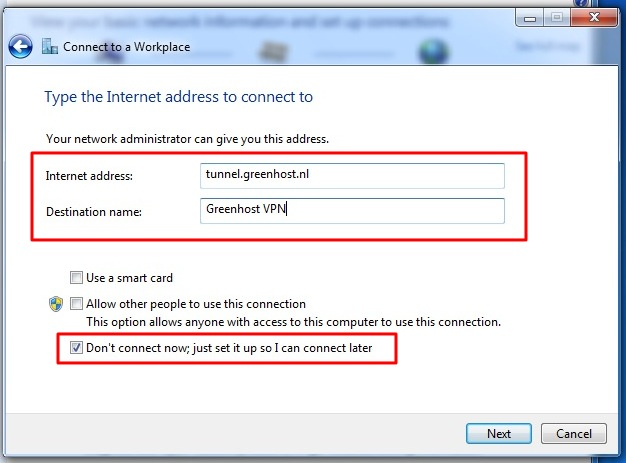
\includegraphics{vpn_windows_05.jpg}
\caption{VPN on Windows}
\end{figure}

\begin{enumerate}[1.]
\setcounter{enumi}{6}
\item
  Next up are your username and password. Just give them like you
  received them from your VPN-provider. If the connection fails, Windows
  forgets them. So keep them with you, you maybe need them later. If
  this is done. Click ``create''.
\end{enumerate}
\begin{figure}[htbp]
\centering
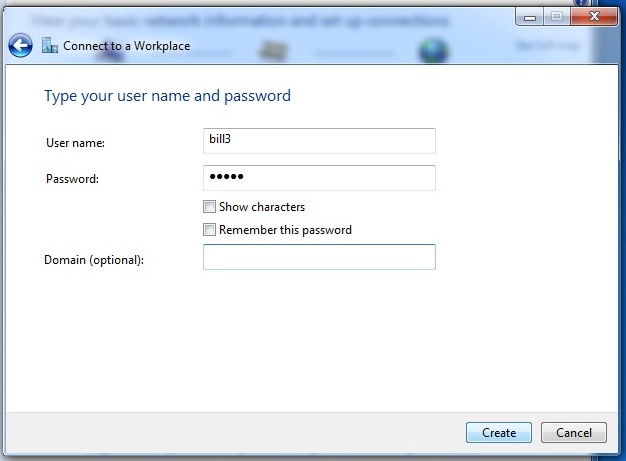
\includegraphics{vpn_windows_06.jpg}
\caption{VPN on Windows}
\end{figure}

\begin{enumerate}[1.]
\setcounter{enumi}{7}
\item
  Your connection is now available, if you click the the network icon
  again, you will see a new option in the network menu, the name of your
  VPN connection, just click it to connect.
\end{enumerate}
\begin{figure}[htbp]
\centering
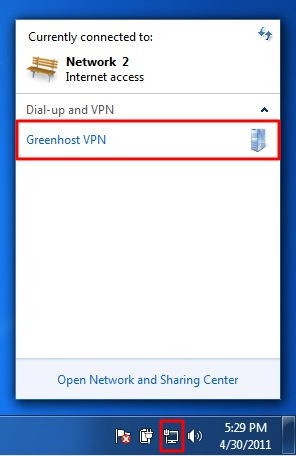
\includegraphics{vpn_windows_07.jpg}
\caption{VPN on Windows}
\end{figure}

\begin{enumerate}[1.]
\setcounter{enumi}{8}
\item
  And click ``connect''
\end{enumerate}
\begin{figure}[htbp]
\centering
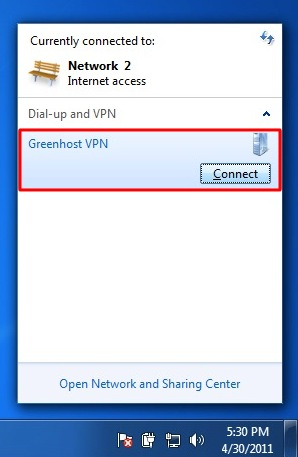
\includegraphics{vpn_windows_08.jpg}
\caption{VPN on Windows}
\end{figure}

\begin{enumerate}[1.]
\setcounter{enumi}{9}
\item
  A VPN connection dialog appears. This give us the opportunity to
  review our settings and to connect. You can try to connect, Windows
  will try to discover all other settings automatically. Unfortunately,
  this does not always work, so if this is not working for you, hit the
  ``properties'' button.
\end{enumerate}
\begin{figure}[htbp]
\centering
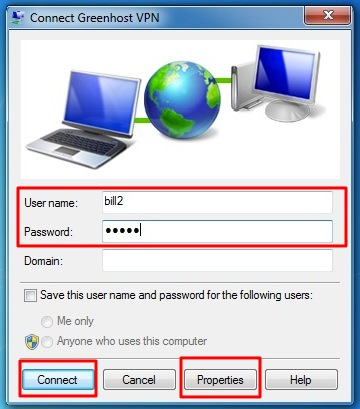
\includegraphics{vpn_windows_09.jpg}
\caption{VPN on Windows}
\end{figure}

\begin{enumerate}[1.]
\setcounter{enumi}{10}
\item
  The properties windows appear. The most important page is the
  ``Security'' page, click on the Security tab to open it.
\end{enumerate}
\begin{figure}[htbp]
\centering
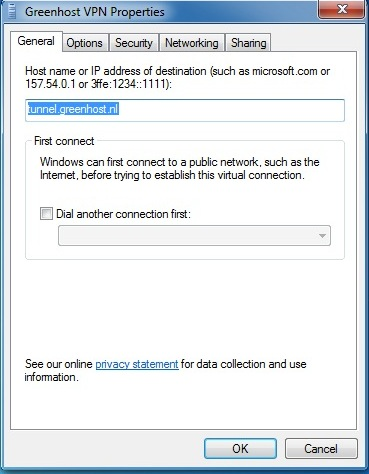
\includegraphics{vpn_windows_10.jpg}
\caption{VPN on Windows}
\end{figure}

\begin{enumerate}[1.]
\setcounter{enumi}{11}
\item
  In the security tab you can specify VPN type, normally L2TP/IPSec. Do
  not use PPTP as it has several security vulnerabilities. For
  L2TP/IPSec also have a look at the Advanced settings.
\end{enumerate}
\begin{figure}[htbp]
\centering
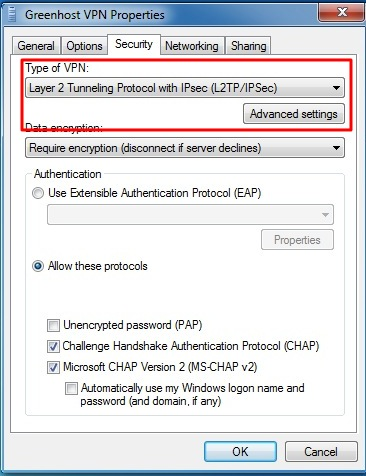
\includegraphics{vpn_windows_11.jpg}
\caption{VPN on Windows}
\end{figure}

\begin{enumerate}[1.]
\setcounter{enumi}{12}
\item
  In the Advanced Settings window, you can specify if you are using a
  pre-shared key or a certificate. This depends on your VPN-provider. If
  you have received a pre-shared-key, Select this option and fill in
  this key. Hit ok afterwards. You will return to the previous window,
  click ok there also
\end{enumerate}
\begin{figure}[htbp]
\centering
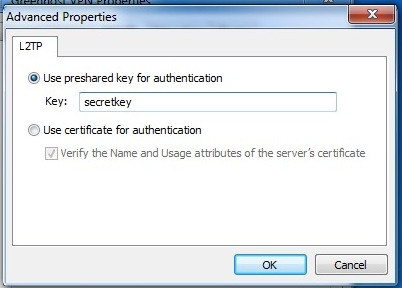
\includegraphics{vpn_windows_12.jpg}
\caption{VPN on Windows}
\end{figure}

\begin{enumerate}[1.]
\setcounter{enumi}{13}
\item
  Back in to connection window try to connect now. Please be sure your
  username and password are filled out.
\end{enumerate}
\begin{figure}[htbp]
\centering
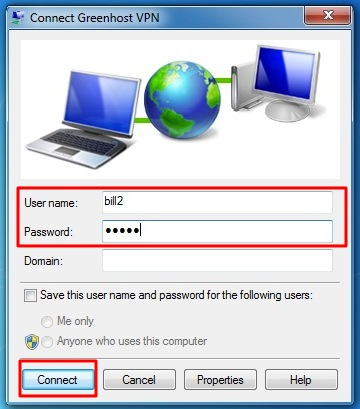
\includegraphics{vpn_windows_13.jpg}
\caption{VPN on Windows}
\end{figure}

\begin{enumerate}[1.]
\setcounter{enumi}{14}
\item
  A connection popup will appear
\end{enumerate}
\begin{figure}[htbp]
\centering
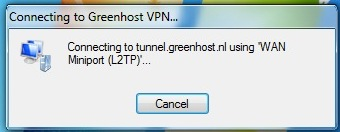
\includegraphics{vpn_windows_14.jpg}
\caption{VPN on Windows}
\end{figure}

\begin{enumerate}[1.]
\setcounter{enumi}{15}
\item
  Online! Don't forget to check if your VPN is working properly.
\end{enumerate}
